%=======================================================================
% SM 4/2017
% Master's thesis Report IISER Thiruvananthapuram
% Investigations of SpinTaylorF2
%=======================================================================

\chapter{Bounds on astrophysical parameters}

Given the two harmonics that capture most of the SNR over a large, but
complimentary regions of the parameter space, naturally leads to 3 possible
cases---the first two, where either $m=0$ mode or $m=2$ dominates over the
other, and the third, where both of these modes have comparable contribution
to the total SNR. Taking into account these 3 possibilities, we divided the
entire $(\theta_J, \kappa)$ parameter space into 3 regions (a, b and c) that
correpond to strongly precessing, moderately precessing, or midly
(non)-precessing systems. 

\begin{figure}[!bp]
\centering
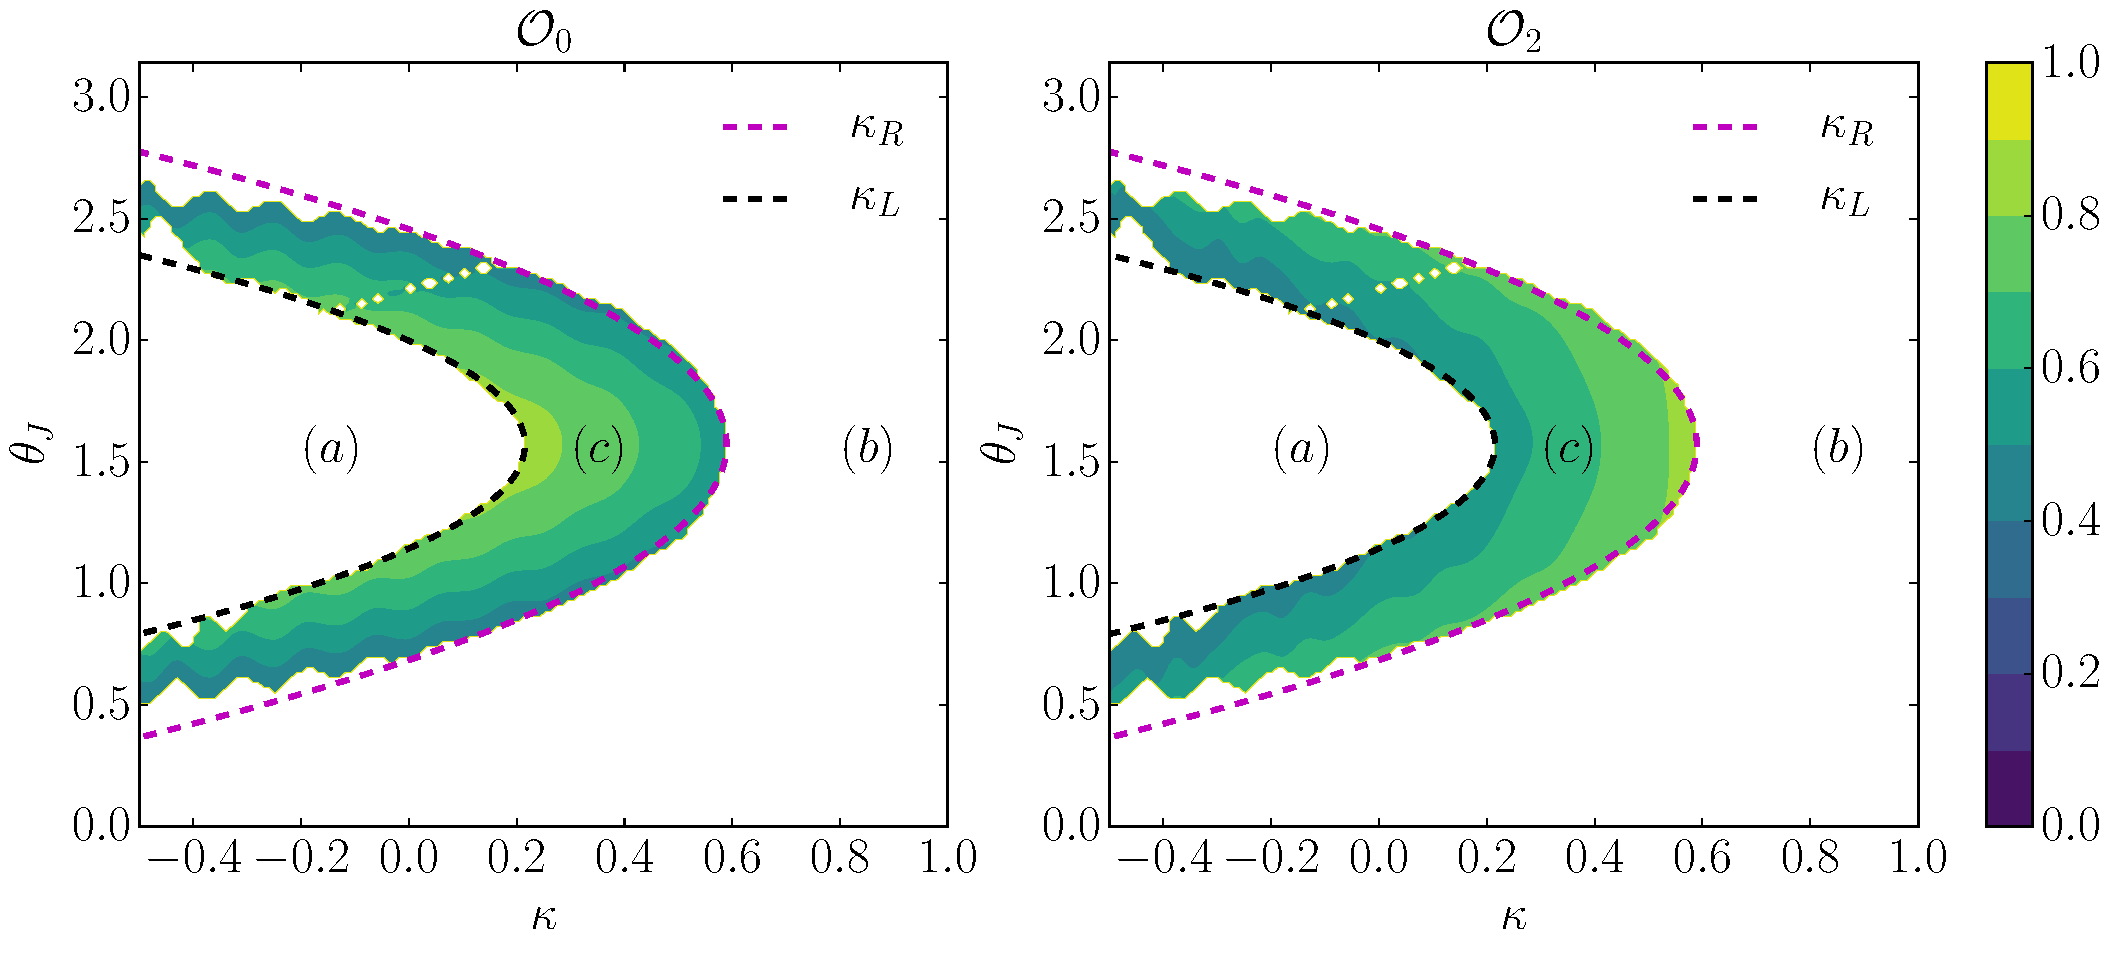
\includegraphics[width=0.8\linewidth]{images/OVLP_cut.pdf}
\caption{\small{Comparison of the overlaps, ${\cal{O}}_2$ and ${\cal{O}}_0$
for ${\cal{O}}_2, ~{\cal{O}}_0 > 0.4$ in the $(\theta_J, \kappa)$ parameter
space, for $m_{1}=14M_{\odot}$ and $\chi_1=0.8$. The three regions: region~(a)
where ${\cal{O}}_0 - {\cal{O}}_2 > 0.3$, region~(b) where ${\cal{O}}_2 -
{\cal{O}}_0 > 0.3$, and regions~(c) where $|{\cal{O}}_2-{\cal{O}}_0|< 0.3$.}}
\label{FIG:OVLP_cut_regions}
\end{figure}

Fig.~\ref{FIG:OVLP_cut_regions} shows these three regions
in the $(\theta_J, \kappa)$ space for a specific NSBH system with $m_{1}=14
M_\odot$, $\chi_1=0.8$, $\psi_J=0.001$ and $\alpha_0 =0.001$. The left panel
and right panel show the contours of ${\cal O}_0$ and ${\cal O}_2$ in
region~(c), respectively. The boundaries of region~(c) correspond
approximately to two parabolas symmetric around $\theta_J=\pi/2$, viz.
\begin{equation}
\kappa = \kappa_{0} - C(\theta_J-\pi/2)^2, 
\label{EQ:boundary_region}
\end{equation}
where $\kappa_0$ and $C$ depend on $\eta$ and $\chi_1$. As the BH mass or spin
increases, the inner boundary that separates region~(b) and region~(c) shifts
$m=2$ mode increases.

\section{Upper bound on $\kappa$}
In the case where the $m=0$ sideband has the largest SNR, one can thus assert that
the system lies in region~(a) in Fig.~\ref{FIG:OVLP_cut_regions}, which
implies that the system is strongly precessing. In such a scenario, using
numerical fits for the boundaries of these regions, one can put an upper bound
on the value of $\kappa$. For example, Fig.~\ref{FIG:kappa_max_bounds} shows
the allowed values for $\kappa$ when $m_1 = 14 M_{\odot}$ or $\eta=0.08$.
Note that even for $\chi_1=1$ (highest possible BH spin), there exists an
upper bound on $\kappa
\leq 0.64$.

\begin{figure}[!htbp]
\centering
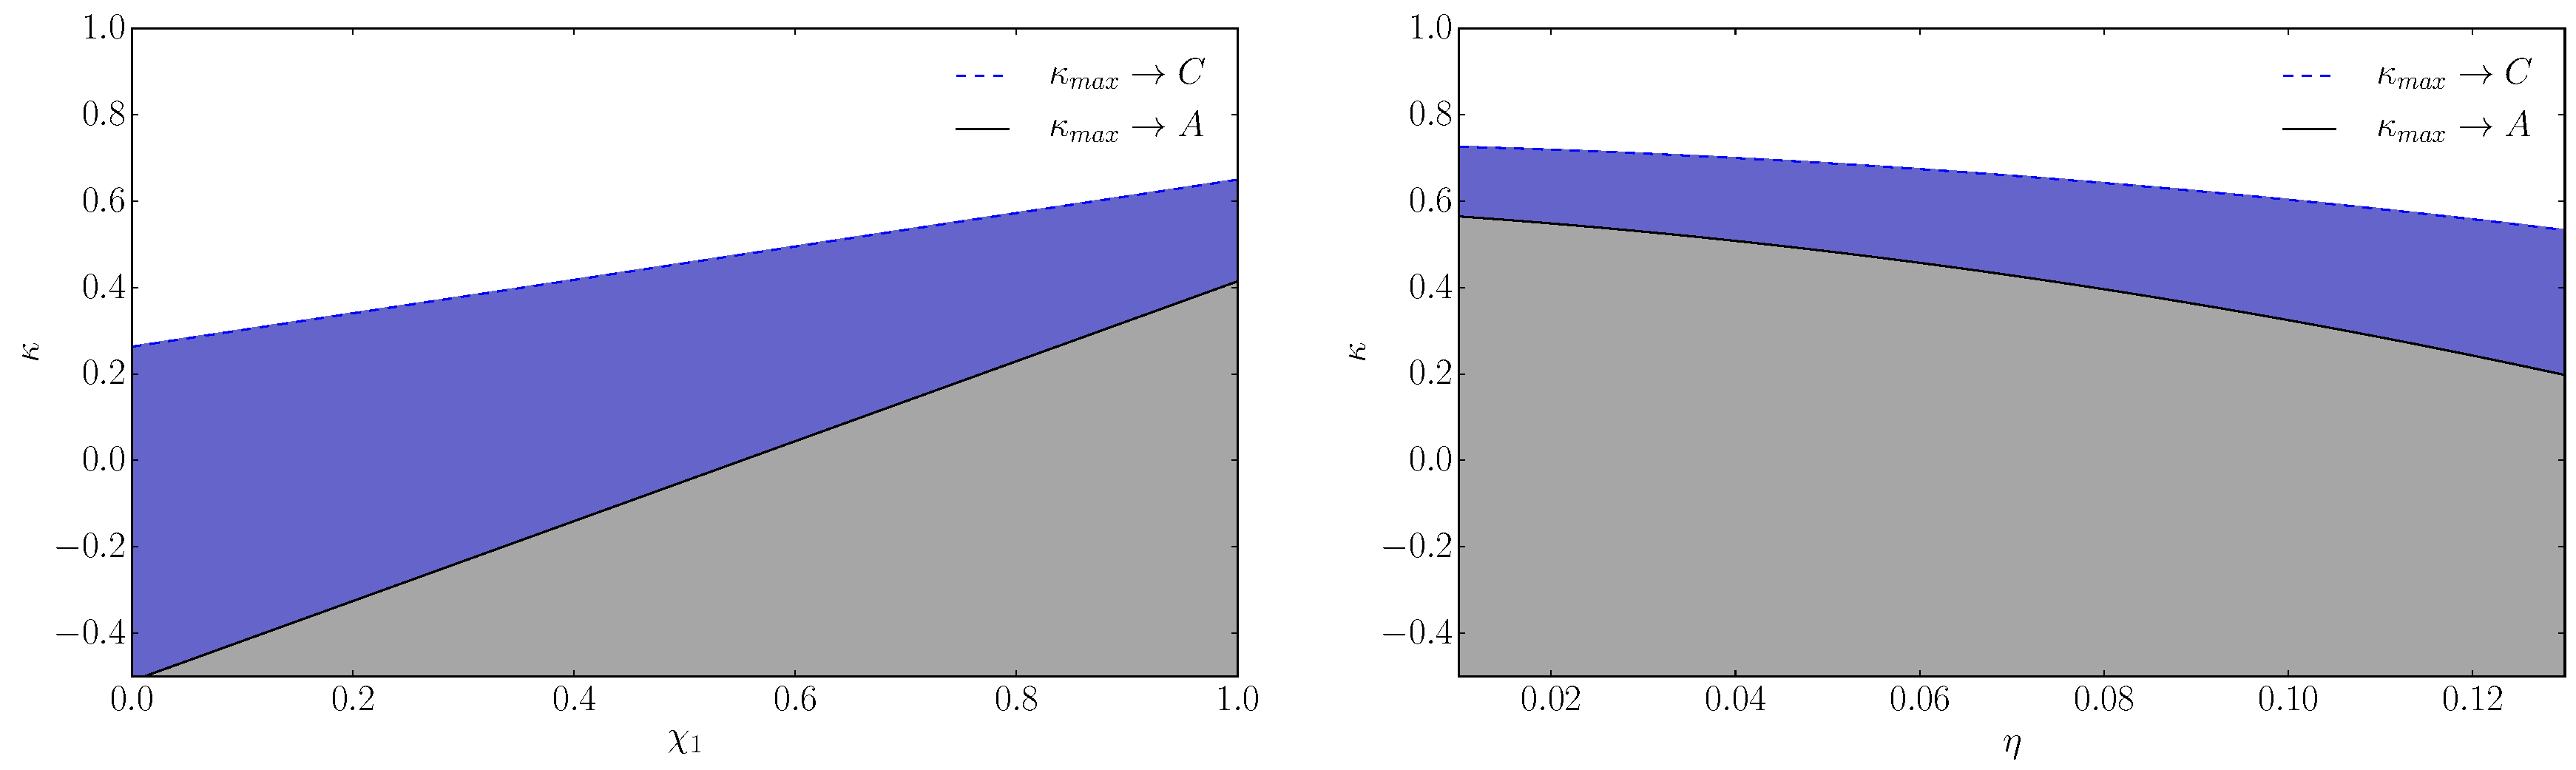
\includegraphics[width=0.65\linewidth]{images/kappa_max_bound.pdf} 
\caption{\small{The dashed line corresponds to the maximum value of $\kappa$ for
    a strongly precessing system, i.e, region~(a) and moderately precessing
    systems that lie in region~(b) in Fig.~\ref{FIG:OVLP_cut_regions}, for
    $m_1 = 14 M_{\odot}$ or $\eta=0.08$. The shaded region represents the
    allowed values of $\kappa$ for a given $\chi_1$. For $\chi_1=1$, $\kappa
    \lesssim 0.64$.}}
\label{FIG:kappa_max_bounds}
\end{figure}